\chapter{Risultati}\label{chapter:res}
I risultati ottenuti utilizzando questo framework ci portano ad effettuare alcune riflessioni. 

Innanzitutto, analizziamo lo spazio di ricerca considerato. Come si può dedurre da Fig. \ref{fig:parallelepipedo} viene ristretto lo spazio di ricerca delle possibile nuove soluzioni il più possibile per non cadere in percorsi troppo complessi. I due centroidi, colorati di rosso, ci dicono dove sono posizionate le parti mobili nello spazio centrate intorno al punto (0,0,0). Tutto sommato lo spazio di ricerca rimane ampio, però per come vengono penalizzati i singoli archi quando cercano di prendere un percorso che si allontana dal segmento ideale che passa in mezzo ai due centroidi riusciamo a mantenere lo spazio esplorato contenuto.  

\begin{figure}[H]
	\centering
	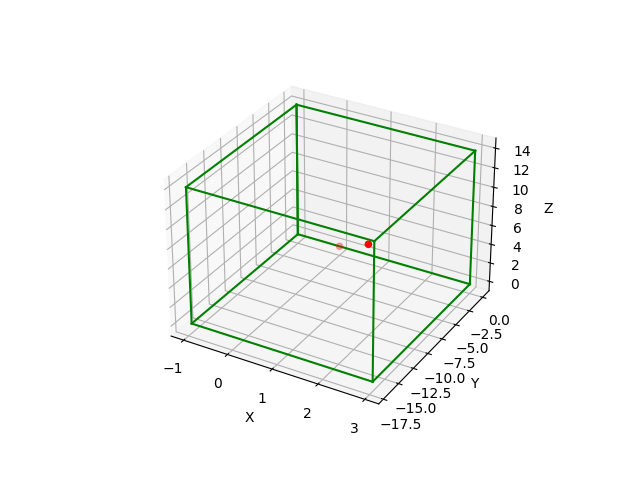
\includegraphics[width=0.6\textwidth]{Immagini/Parallelepipedo.png}
	\caption{In rosso sono riportati i centroidi delle due configurazioni che stiamo analizzando, mentre in verde evidenziamo il parallelepipedo che racchiude lo spazio di ricerca.}
	\label{fig:parallelepipedo}
\end{figure} 

Idealmente esiste come percorso ottimo quello che appunto segue il segmento tra i due centroidi. Infatti testando la fattibilità del percorso abbiamo ottenuto il seguente risultato Fig. \ref{fig:movimento}.

\begin{figure}[H]
	\centering
	\subfloat[][\emph{Vicinato d'esplorazione}]
	{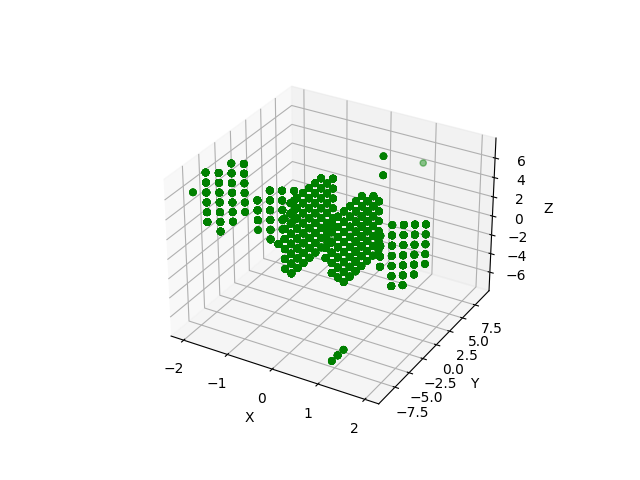
\includegraphics[width=0.5\textwidth]{Immagini/Sequenza_transizioni.png}} 
	\subfloat[][\emph{Percorso minimo pratico}]
	{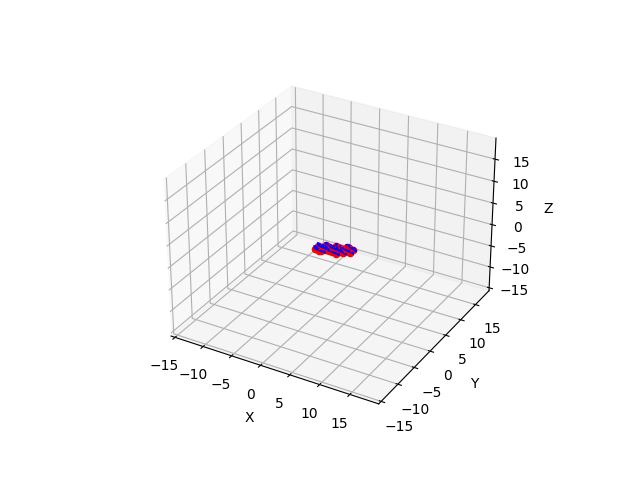
\includegraphics[width=0.6\textwidth]{Immagini/Movimento.png}}
	\caption{In (\textbf{a}) viene mostrato il vicinato d'esplorazione; mentre in (\textbf{b}) viene mostrato il percorso pratico minimo.}
	\label{fig:movimento}
\end{figure}

Come è possibile notare in effetti non ci si allontana molto dalla segmento ideale che connette i due centroidi, l'unica differenza presente è l'evoluzione a scaletta data dall'uso del vicinato semplice, come visto in Fig. \ref{fig:Transizioni}(\textbf{a}). 

Si può notare anche l'evoluzione del vicinato di esplorazione, prodotto da shortest path, si aggira intorno a quello che è il segmento teorico che unisce i due centroidi a riprova della corretta valutazione del costo per ogni nodo.

Finora è stata dimostrata la fattibilità teorica e pratica di convergere dalla conformazione chiusa alla conformazione aperta, il tutto senza verificare che ogni nuova parte mobile generata fosse raggiungibile dai loop. Prima di verificare come cambiano i risultati descritti in precedenza cercando convergenza anche con i loop è necessario esaminare come ogni loop crei un collegamento stabile  con la nuova configurazione intermedia. 
